% ======================================================================
% col: 20

\chapter{Implementazione}
In questo capitolo verranno descritti i passaggi implementati per generare la raceline ottima data una
mappa.

Il lavoro svolto è stato basato sulla seguente repository GitHub:
\url{https://github.com/CL2-UWaterloo/Raceline-Optimization}.

\bigskip
\noindent I passaggi ad alto livello sono i seguenti:
\begin{enumerate}
	\item Ottenere l'immagine di una mappa (per esempio attraverso \hyperref[par:slam]{SLAM});
	\item Eventualmente ripurla di imperfezioni e ottenere un circuito chiuso; 
	\item Generare la centerline e calcolare la larghezza del circuito;
	\item Applicare gli algoritmi di generazione della raceline;
\end{enumerate}

%TODO:spiegare occupancy grid?
La mappa digitalizzata in file immagine che rappresenta una occupancy grid, mentre
i percorsi, che siano raceline o centerline, sono in formato csv con almeno due colonne rappresentanti la
posizione $(x,y)$ di ogni sample e almeno una terza colonna per la velocità per quanto riguarda la
raceline. Successivamente si è scelto di esportare anche l'orientamento del robot rispetto alla mappa e
l'accelerazione per ogni sample.

\section{Generazione centeline}
Affinchè l'algoritmo per l'estrazione della linea di riferimento restituisca un risultato corretto, come
detto in precedenza, l'immagine della mappa deve rappresentare un circuito chiuso e con bordi ben
definiti e lisci, come effettivamente sarebbe un circuito di F1.
Dunque se si acquisice una mappa con SLAM come in figura \ref{fig:slam_map} è necessario modificarla come
in figura \ref{fig:slam_map_mod}. Durante l'implentazione di questa tesi si è deciso di usare le mappe
dei circuiti da gara più famosi forniti da F1TENTH stesso \cite{f1tenth-gitmaps}.

\begin{figure}[H]
	\begin{minipage}[c]{0.47\textwidth}
		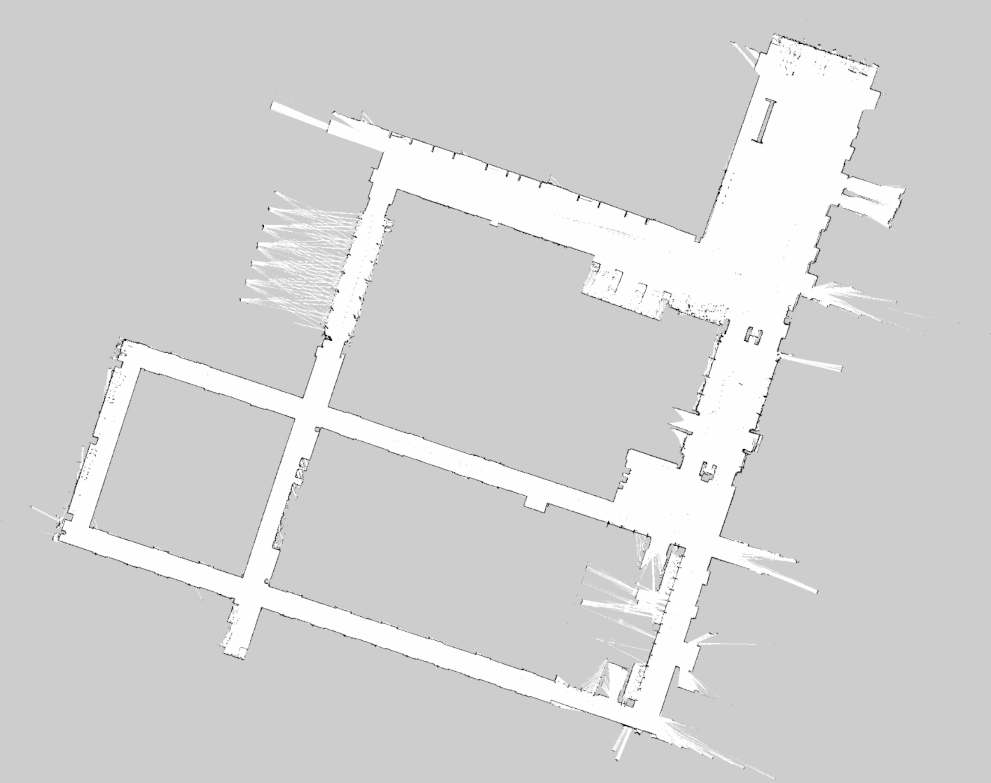
\includegraphics[width=1\textwidth]{slam_map.png}
		\caption{\raggedright Mappa risultante da SLAM}
		\label{fig:slam_map}
	\end{minipage}\hfill
	\begin{minipage}[c]{0.47\textwidth}
		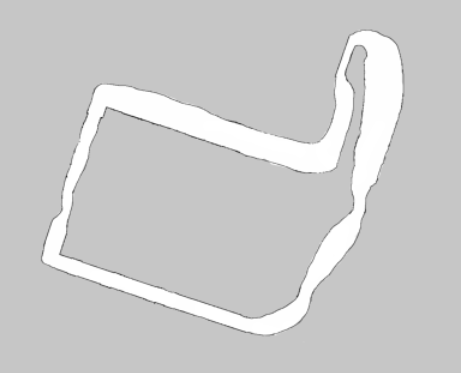
\includegraphics[width=1\textwidth]{slam_map_mod.png}
		\caption{Modifica dell'immagine \ref{fig:slam_map} per creare un circuito chiuso}
		\label{fig:slam_map_mod}
	\end{minipage}
\end{figure}

Operativamente, l'algoritmo usato per la generazione viene dal mondo dell'elaborazione delle immagini e
si chiama EDT (Euclidian Distance Transform), che calcola la distanza euclidea per ogni pixel
dell'immagine dal background: in questo caso, lo sfondo preso in considerazione sono i punti non
esplorati, ovvero quelli esterni ai bordi del circuito.
Un esempio di applicazione di EDT si trova all'immagine \ref{fig:edt-ex}.

% \begin{figure}[h]
% 	\begin{minipage}[c]{1\textwidth}
% 		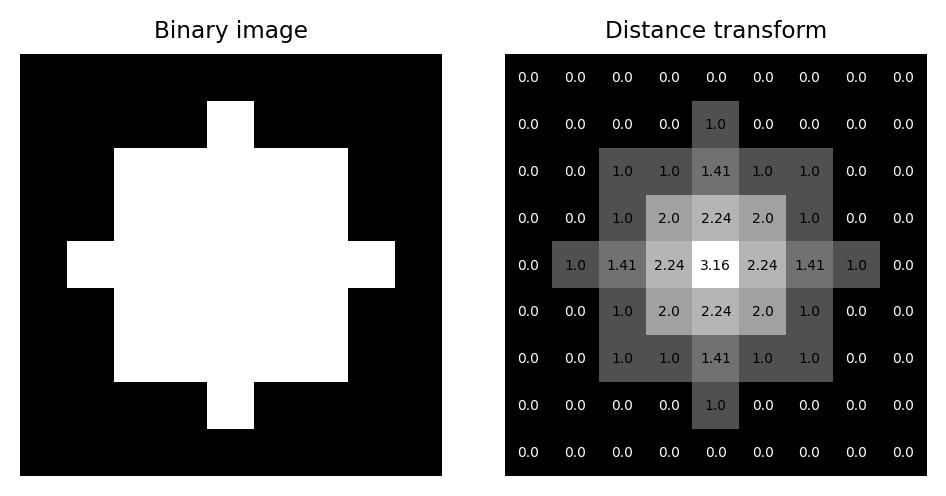
\includegraphics[width=1\textwidth]{edt-ex.png}
% 		\caption{Esempio di applicazione dell'agortimo EDT su una immagine binaria, l'immagine a destra
% 		mostra il risultato indicando la distanza euclidea dal background per ogni pixel}
% 		\label{fig:edt-ex}
% 	\end{minipage}\hfill
% \end{figure}

Un aspetto da sottolineare è che le immagini fornite da F1TENTH rappresentano una occupancy grid
ternaria, in cui il grigio corrisponde alle zone non esplorate; per sfruttare l'algoritmo sopra citato è
necessario che i pixel grigi vengano convertiti in nero, perchè  è il valore considerato come background
dall'algoritmo EDT. Prendendo come riferimento il circuito di Monza all'immagine \ref{fig:monza-binary}, il
risultato dell'algoritmo si può vedere all'immagine \ref{fig:monza-edt}.

\begin{figure}[H]
	\begin{minipage}[c]{1\textwidth}
		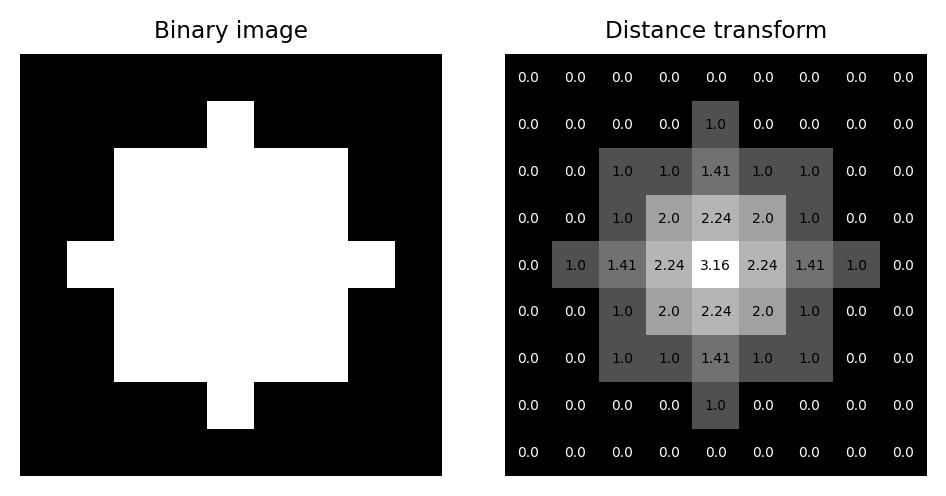
\includegraphics[width=1\textwidth]{edt-ex.png}
		\caption{Esempio di applicazione dell'agortimo EDT su una immagine binaria, l'immagine a destra
		mostra il risultato indicando la distanza euclidea dal background per ogni pixel}
		\label{fig:edt-ex}
	\end{minipage}\hfill
	\vspace{1cm}
	\begin{minipage}[c]{0.47\textwidth}
		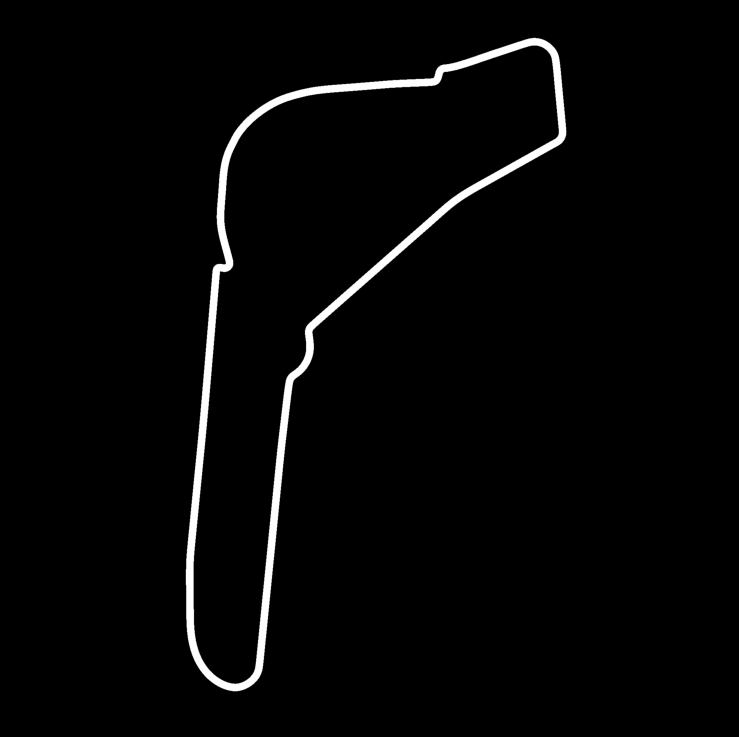
\includegraphics[width=1\textwidth]{monza-binary.png}
		\caption{Immagine della occupancy grid binaria del circuito di Monza}
		\label{fig:monza-binary}
	\end{minipage}\hfill
	\begin{minipage}[c]{0.47\textwidth}
		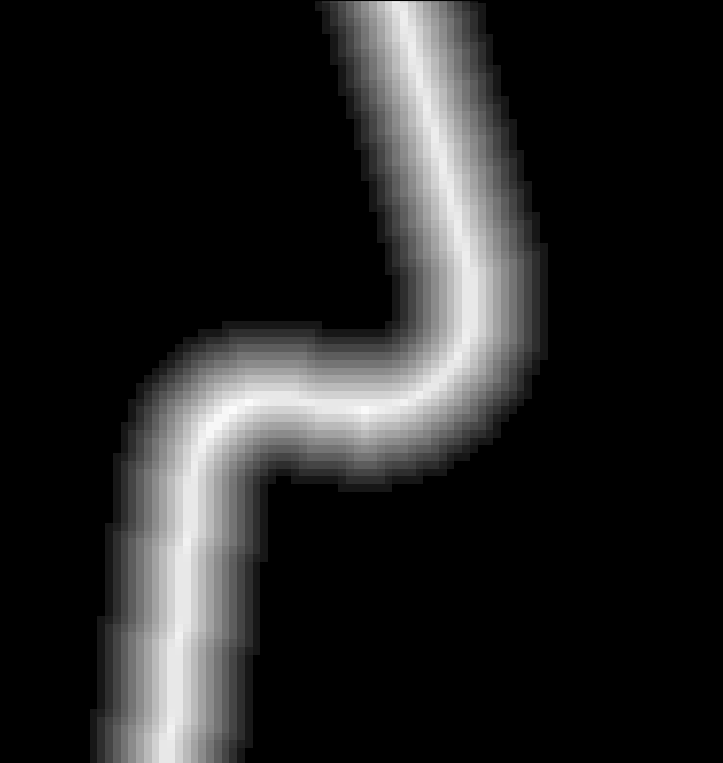
\includegraphics[width=1\textwidth]{monza-edt.png}
		\caption{\raggedright Risultato dell'algoritmo EDT mostrato sulla curva 1-2 del circuito di Monza}
		\label{fig:monza-edt}
	\end{minipage}
\end{figure}

Il passo successivo è quello di ottenere solo la parte centrale, ovvero quella con i valori di bianco
più alti e ridurla a un singolo pixel. In Python, questa operazione, viene eseguita dalla funzione
\verb|skeletonize()| del pacchetto \verb|scikit-image|. Seguendo l'esempio con il circuito di Monza, il
risultato di questa fase si può osservare all'immagine \ref{fig:monza-skel}.

A questo punto è necessario campionare il percorso di un pixel trovato: partendo da un punto del
percorso, si applica una ricerca DFS (Depth First Search) per trovare i successivi pixel bianchi. Dunque
da un pixel del percorso, si cerca il primo pixel bianco in tutte le direzioni che non sia già stato
esplorato: seguendo questo processo si ottengono le posizioni dei pixel e la loro distanza dai bordi, si
trasformano nel frame della mappa e esportano queste informazioni in un csv contentente le colonne
\verb|x, y, width_left, width_right|.

\begin{figure}[h]
	\begin{center}
		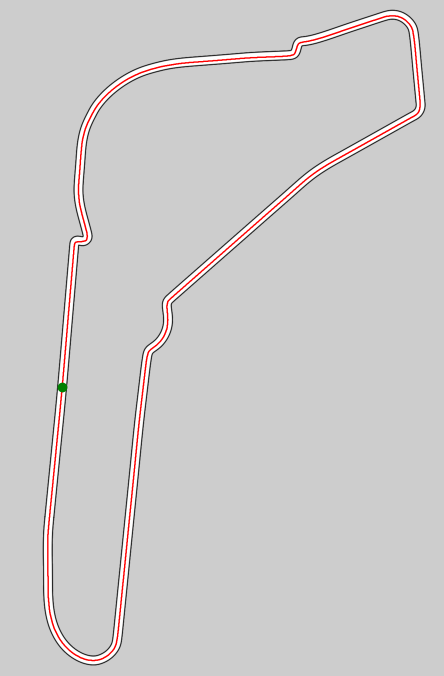
\includegraphics[width=0.3\textheight]{monza-skel.png}
	\end{center}
	\caption{Visualizzazione della centerline di Monza, il punto verde indica il punto di partenza}\label{fig:monza-skel}
\end{figure}


\section{Esecuzione dell'ottimizzazione}
Ad alto livello, l'ottimizzazione cerca iterativamente di aggiustare la centerline in modo tale da
ottenere il risultato migliore, come spiegato nel capitolo \ref{chap:opt} (pag. \pageref{chap:opt}).
Questa fase non richiede solamente di eseguire il programma solutore, ma è necessario
configurare i parametri che l'algortimo usa. Questo compito si chiama \textit{tuning} dei parametri
e consiste nel trovare quelli che meglio si adattano nel trovare la soluzione migliore.

Durante lo studio di questa tesi il principale parametro modificato durante le prove è stato lo
\textit{stepsize}, ovvero la distanza, in metri, tra un sample e l'altro. In particolare si distinguono
tre stepsize diversi:
\begin{itemize}
	\item \verb|stepsize_prep|: viene usato per l'interpolazione lineare prima dell'approssimazione del
		percorso con la spline;
	\item \verb|stepsize_reg|: usato durante l'ottimizzazione per l'interpolazione della spline;
	\item \verb|stepsize_interp_after_opt|: usato per campionare la spline dopo l'ottimizzaione e da esportare in csv;
\end{itemize}

\noindent Altri parametri fanno riferimento alla dinamica del veicolo, come accelerazione massima e velocità
massima, e grandezze fisiche del veicolo, come massa, lunghezza e larghezza compresa on un margine di
sicurezza aggiuntivo. 

\begin{figure}
	\begin{center}
		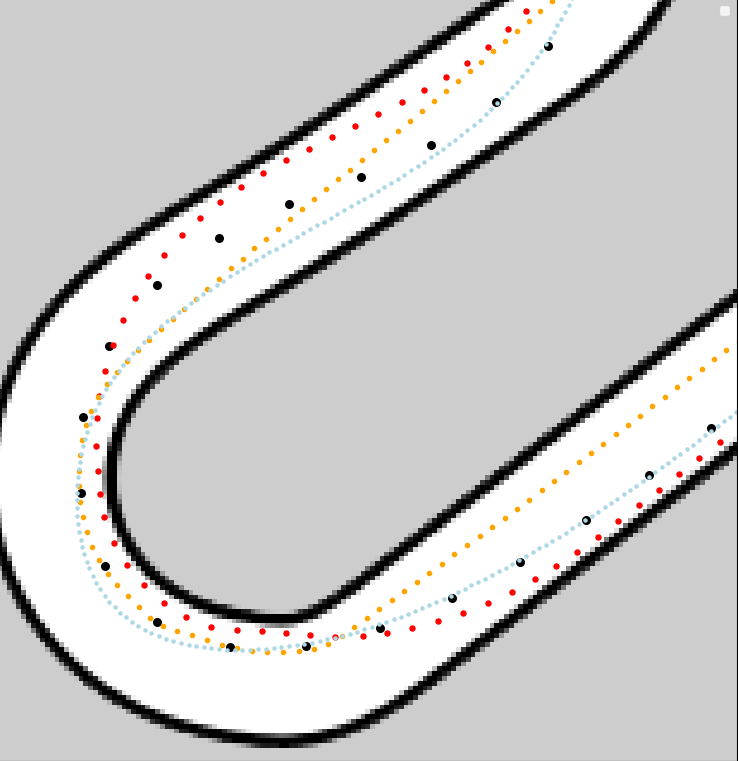
\includegraphics[width=0.75\textwidth]{stepsize.png}
	\end{center}
	\caption{Quattro traiettorie con stepsize diversi: nera a 1.5m, rossa a 0.5m, arancione a 0.3m e azzurra a 0.15m}
	\label{fig:stepsize}
\end{figure}


È facile immaginare che una minore distanza tra i sample durante l'ottimizzazione indichi un risultato
più preciso a costo di aumentare la complessità computazionale e anche il tempo di esecuzione. In figura
\ref{fig:stepsize} si visualizza una comparazione tra raceline con stepsize diversi.

% TODO: palare della parte del notebook
